% Paquets généraux
\documentclass[a4paper,12pt,titlepage]{article}
\usepackage[T1]{fontenc}
\usepackage[utf8]{inputenc}
\usepackage[french]{babel}
\usepackage[gen]{eurosym}
%\usepackage[dvips]{graphicx}
\usepackage{fancyhdr}
\usepackage{pdfpages} 
\usepackage{multido}
\usepackage{hyperref}
%\usepackage{textcomp}
%\usepackage{aeguill}
\usepackage{schemabloc}
\usepackage[bitstream-charter]{mathdesign}

\newcommand{\id}{54}
\newcommand{\nom}{Liaisons mécaniques}
\newcommand{\sequence}{04}
\newcommand{\num}{01}
\newcommand{\type}{TP}
\newcommand{\descrip}{Modélisation d'un solide. Comportement des liaisons mécaniques. Modéliser les mécanismes du laboratoire par un schéma cinématique, paramétré.}
\newcommand{\competences}{A3-C4: Analyse d'architecture et de comportement \\ &  Mod1-C1: Isolement d'un solide ou d'un système de solides \\ &  Mod2-C10-1: Modèle de solide indéformable \\ &  Mod2-C11: Modélisation géométrique et cinématique des mouvements entre solides indéformables \\ &  Mod2-C12: Modélisation cinématique des liaisons entre solides \\ &  Mod2-C15: Modélisation des actions mécaniques \\ &  Rés-C6: Utilisation d'un solveur ou d'un logiciel multi physique \\ &  Com1-C1: Différents descripteurs introduits dans le programme \\ &  Com2-C4: Outils de communication}
\newcommand{\nbcomp}{9}
\newcommand{\systemes}{Plateforme Stewart}
\newcommand{\systemessansaccent}{Plateforme Stewart}
\newcommand{\ilot}{2}
\newcommand{\ilotstr}{02}
\newcommand{\dossierilot}{\detokenize{Ilot_02 Plateforme Stewart}}
\newcommand{\imageun}{Plateforme}

\newcommand{\urlsysteme}{\href{https://www.costadoat.fr/systeme/57}{Ressources système}}
\newcommand{\matlabsimscape}{\href{https://github.com/Costadoat/Sciences-Ingenieur/raw/master/Systemes/Plateforme Stewart/Plateforme_Stewart_Simscape.zip}{Modèle Simscape}}
\newcommand{\solidworks}{\href{https://github.com/Costadoat/Sciences-Ingenieur/raw/master/Systemes/Plateforme Stewart/Plateforme_Stewart_Solidworks.zip}{Modèle Solidworks}}
\newcommand{\edrawings}{\href{https://github.com/Costadoat/Sciences-Ingenieur/raw/master/Systemes/Plateforme Stewart/Plateforme_Stewart.EASM}{Modèle eDrawings}}
\newcommand{\test}{Stewart_param1}
\newcommand{\testi}{Stewart_param2}
\newcommand{\testii}{Stewart_param3}
\newcommand{\testiii}{Stewart_param4}
\newcommand{\testiiii}{Stewart_euler}

\newcommand{\auteurun}{Renaud Costadoat}
\newcommand{\auteurdeux}{Françoise Puig}
\newcommand{\institute}{Lycée Dorian}


\usepackage{color}
\usepackage{xcolor}
\usepackage{colortbl}
\usepackage{helvet}
\renewcommand{\familydefault}{\sfdefault}
\usepackage{amsfonts}
\usepackage{amsmath}
%\usepackage{xspace}
\usepackage{varioref}
\usepackage{tabularx}
%\usepackage{floatflt}
\usepackage{graphics}
\usepackage{wrapfig}
\usepackage{textcomp}
\usepackage{tikz}
\usepackage{wrapfig}
\usepackage{gensymb}
\usepackage[european]{circuitikz}
\usetikzlibrary{babel}
\usepackage{ifthen}
\usepackage{cancel}
\usepackage{etoolbox}
\usepackage{multirow}
%\usepackage{boxedminipage}
\definecolor{gris25}{gray}{0.75}
\definecolor{bleu}{RGB}{18,33,98}
\definecolor{bleuf}{RGB}{42,94,171}
\definecolor{bleuc}{RGB}{231,239,247}
\definecolor{rougef}{RGB}{185,18,27}
\definecolor{rougec}{RGB}{255,188,204}%255,230,231
\definecolor{vertf}{RGB}{103,126,82}
\definecolor{vertc}{RGB}{220,255,191}
\definecolor{forestgreen}{rgb}{0.13,0.54,0.13}
\definecolor{blcr}{rgb}{0.59,0.69,0.84}
\definecolor{blfr}{rgb}{0.32,0.51,0.75}
\definecolor{orfr}{rgb}{0.90,0.42,0.15}
\definecolor{orcr}{rgb}{0.90,0.65,0.50}
\definecolor{orangef}{rgb}{0.659,0.269,0.072}
\definecolor{orange}{rgb}{0.58,0.35,0.063}
\definecolor{orangec}{rgb}{0.43,0.32,0.25}
\definecolor{rcorrect}{rgb}{0.6,0,0}
\definecolor{sequence}{rgb}{0.75,0.75,0.75}
\definecolor{competences}{rgb}{0.61,0.73,0.35}
\definecolor{grisf}{HTML}{222222}
\definecolor{grisc}{HTML}{636363}
\definecolor{normal}{HTML}{4087c4}
\definecolor{info}{HTML}{5bc0de}
\definecolor{success}{RGB}{92,184,92}
\definecolor{warning}{RGB}{240,173,78}
\definecolor{danger}{RGB}{217,83,79}
\hypersetup{                    % parametrage des hyperliens
    colorlinks=true,                % colorise les liens
    breaklinks=true,                % permet les retours à la ligne pour les liens trop longs
    urlcolor= blfr,                 % couleur des hyperliens
    linkcolor= orange,                % couleur des liens internes aux documents (index, figures, tableaux, equations,...)
    citecolor= forestgreen                % couleur des liens vers les references bibliographiques
    }

% Mise en page
\pagestyle{fancy}

\setlength{\hoffset}{-18pt}

\setlength{\oddsidemargin}{0pt} 	% Marge gauche sur pages impaires
\setlength{\evensidemargin}{0pt} 	% Marge gauche sur pages paires
\setlength{\marginparwidth}{00pt} 	% Largeur de note dans la marge
\setlength{\headwidth}{481pt} 	 	% Largeur de la zone de tête (17cm)
\setlength{\textwidth}{481pt} 	 	% Largeur de la zone de texte (17cm)
\setlength{\voffset}{-18pt} 		% Bon pour DOS
\setlength{\marginparsep}{7pt}	 	% Séparation de la marge
\setlength{\topmargin}{-30pt} 		% Pas de marge en haut
\setlength{\headheight}{35pt} 		% Haut de page
\setlength{\headsep}{20pt} 		% Entre le haut de page et le texte
\setlength{\footskip}{30pt} 		% Bas de page + séparation
\setlength{\textheight}{700pt} 		% Hauteur de l'icone zone de texte (25cm)
\setlength\fboxrule{1 pt}
\renewcommand{\baselinestretch}{1}
\setcounter{tocdepth}{1}
\newcommand{\cadre}[2]
{\fbox{
  \begin{minipage}{#1\linewidth}
   \begin{center}
    #2\\
   \end{center}
  \end{minipage}
 }
}

\newcounter{num_quest} \setcounter{num_quest}{0}
\newcounter{num_rep} \setcounter{num_rep}{0}
\newcounter{num_cor} \setcounter{num_cor}{0}

\newcommand{\question}[1]{\refstepcounter{num_quest}\par
~\ \\ \parbox[t][][t]{0.15\linewidth}{\textbf{Question \arabic{num_quest}}}\parbox[t][][t]{0.93\linewidth}{#1}\par
}


\newcommand{\reponse}[1]
{\refstepcounter{num_rep}
\noindent
\rule{\linewidth}{.5pt}
\textbf{Question \arabic{num_rep}:}
\multido{\i=1+1}{#1}{~\ \\}
}

\newcommand{\cor}
{\refstepcounter{num_cor}
\noindent
\rule{\linewidth}{.5pt}
\textbf{Question \arabic{num_cor}:} \\
}

\newcommand{\titre}[1]
{\begin{center}
\cadre{0.8}{\huge #1} 
\end{center}
}


% En tête et pied de page
\fancypagestyle{normal}{%
  \fancyhf{}
\lhead{\nom}
\rhead{
\includegraphics[width=2cm]{../../img/logo}\hspace{2pt}}
\ifdef{\auteurdeux}{\lfoot{\auteurun,\auteurdeux}}{\lfoot{\auteurun}}
\cfoot{Page \thepage}}

\fancypagestyle{correction}{%
  \fancyhf{}
  \lhead{\colorbox{danger}{\begin{minipage}{0.65\paperwidth} \textcolor{white}{\textbf{Correction}} \end{minipage}} }
  \rhead{
\includegraphics[width=2cm]{../../img/logo}}
  \ifdef{\auteurdeux}{\lfoot{\auteurun,\auteurdeux}}{\lfoot{\auteurun}}
  \rfoot{\colorbox{danger}{\begin{minipage}{0.5\paperwidth} \begin{flushright}\textcolor{white}{\textbf{Correction}}\end{flushright} \end{minipage}} }}

\renewcommand{\footrulewidth}{0.4pt}

\usepackage{eso-pic}
\newcommand{\BackgroundPic}{%
\put(0,0){%
\parbox[b][\paperheight]{\paperwidth}{%
\vfill
\begin{center}
\hspace{0.5cm}\vspace{0.5cm}
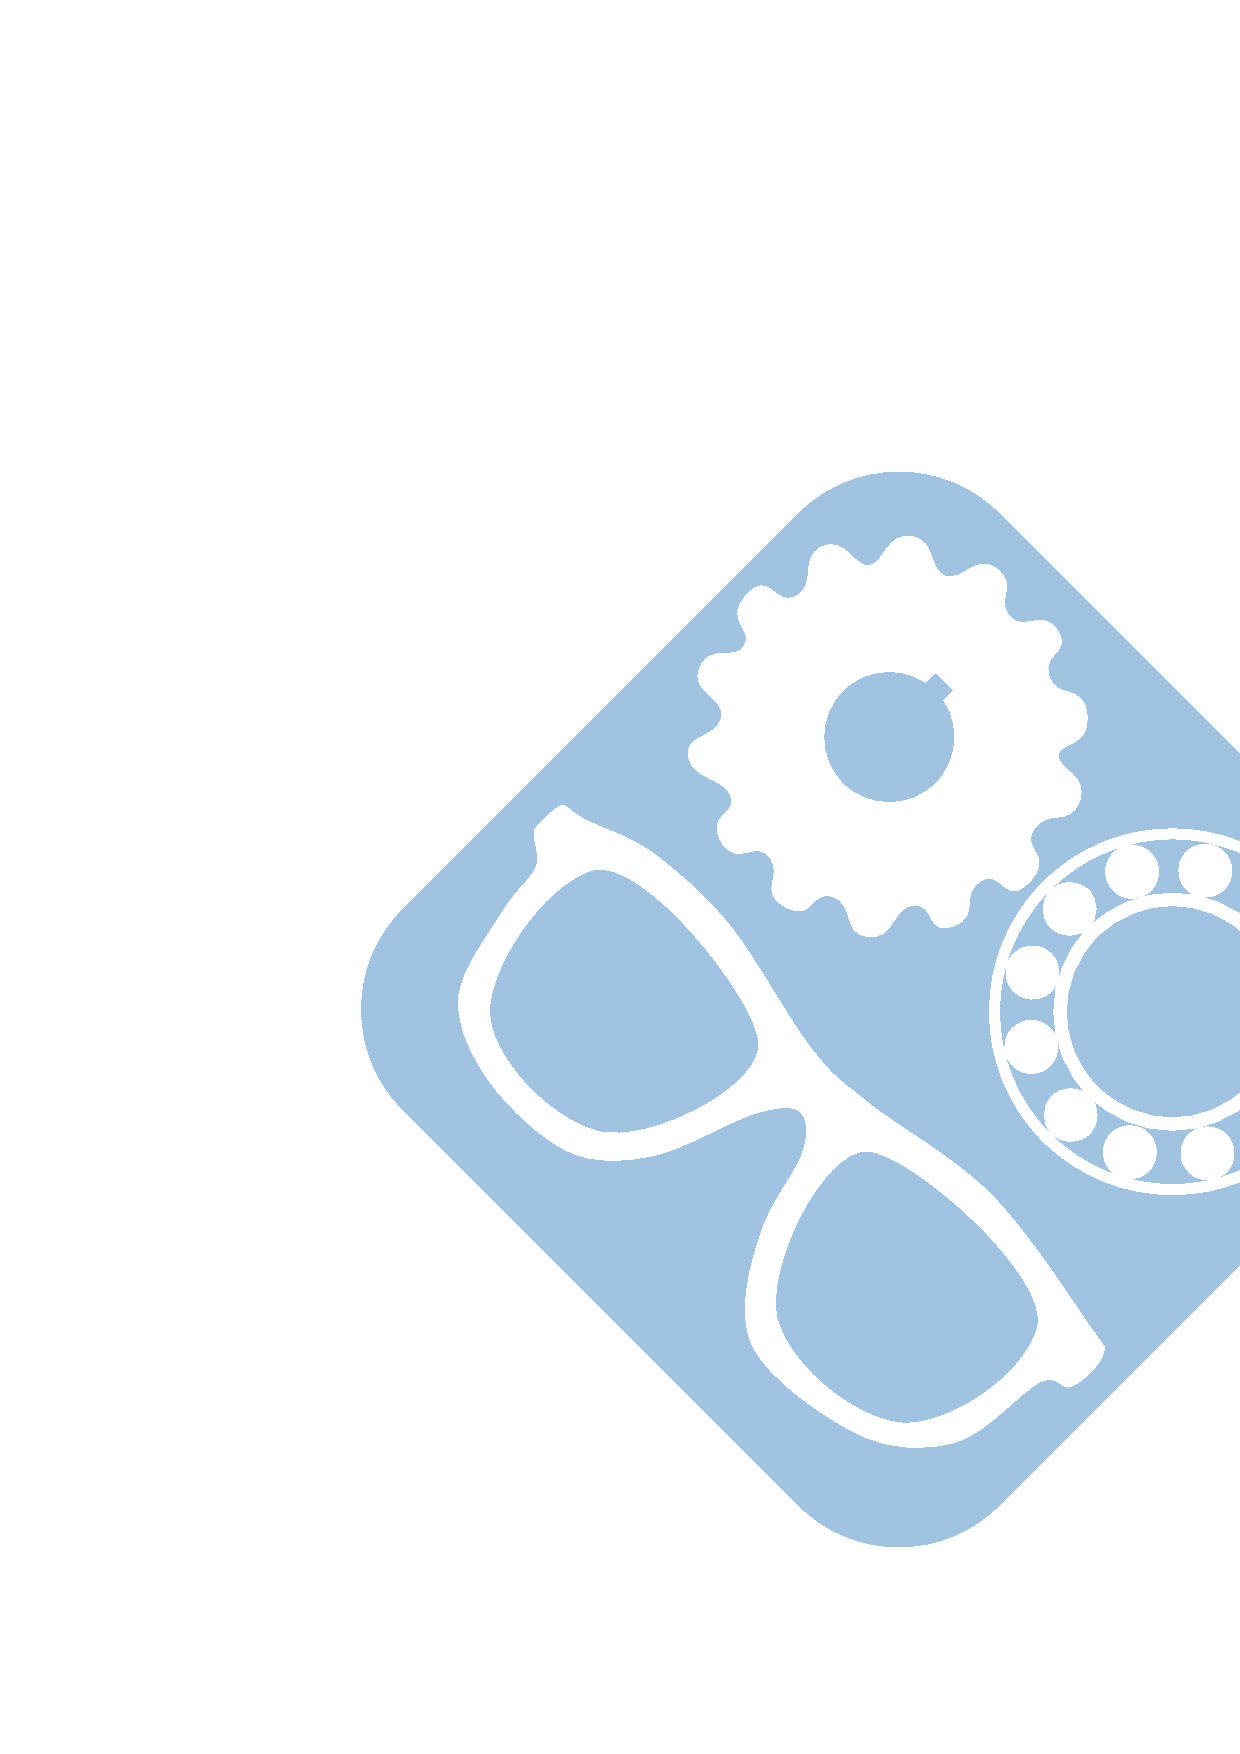
\includegraphics[width=\paperwidth,height=\paperheight,%
keepaspectratio]{../../img/fond3}%
\end{center}
\vfill
}}}

\newcommand{\BackgroundPicdeux}{%
\put(25,-30){%
\parbox[b][\paperheight]{\paperwidth}{%
\vfill
\begin{center}
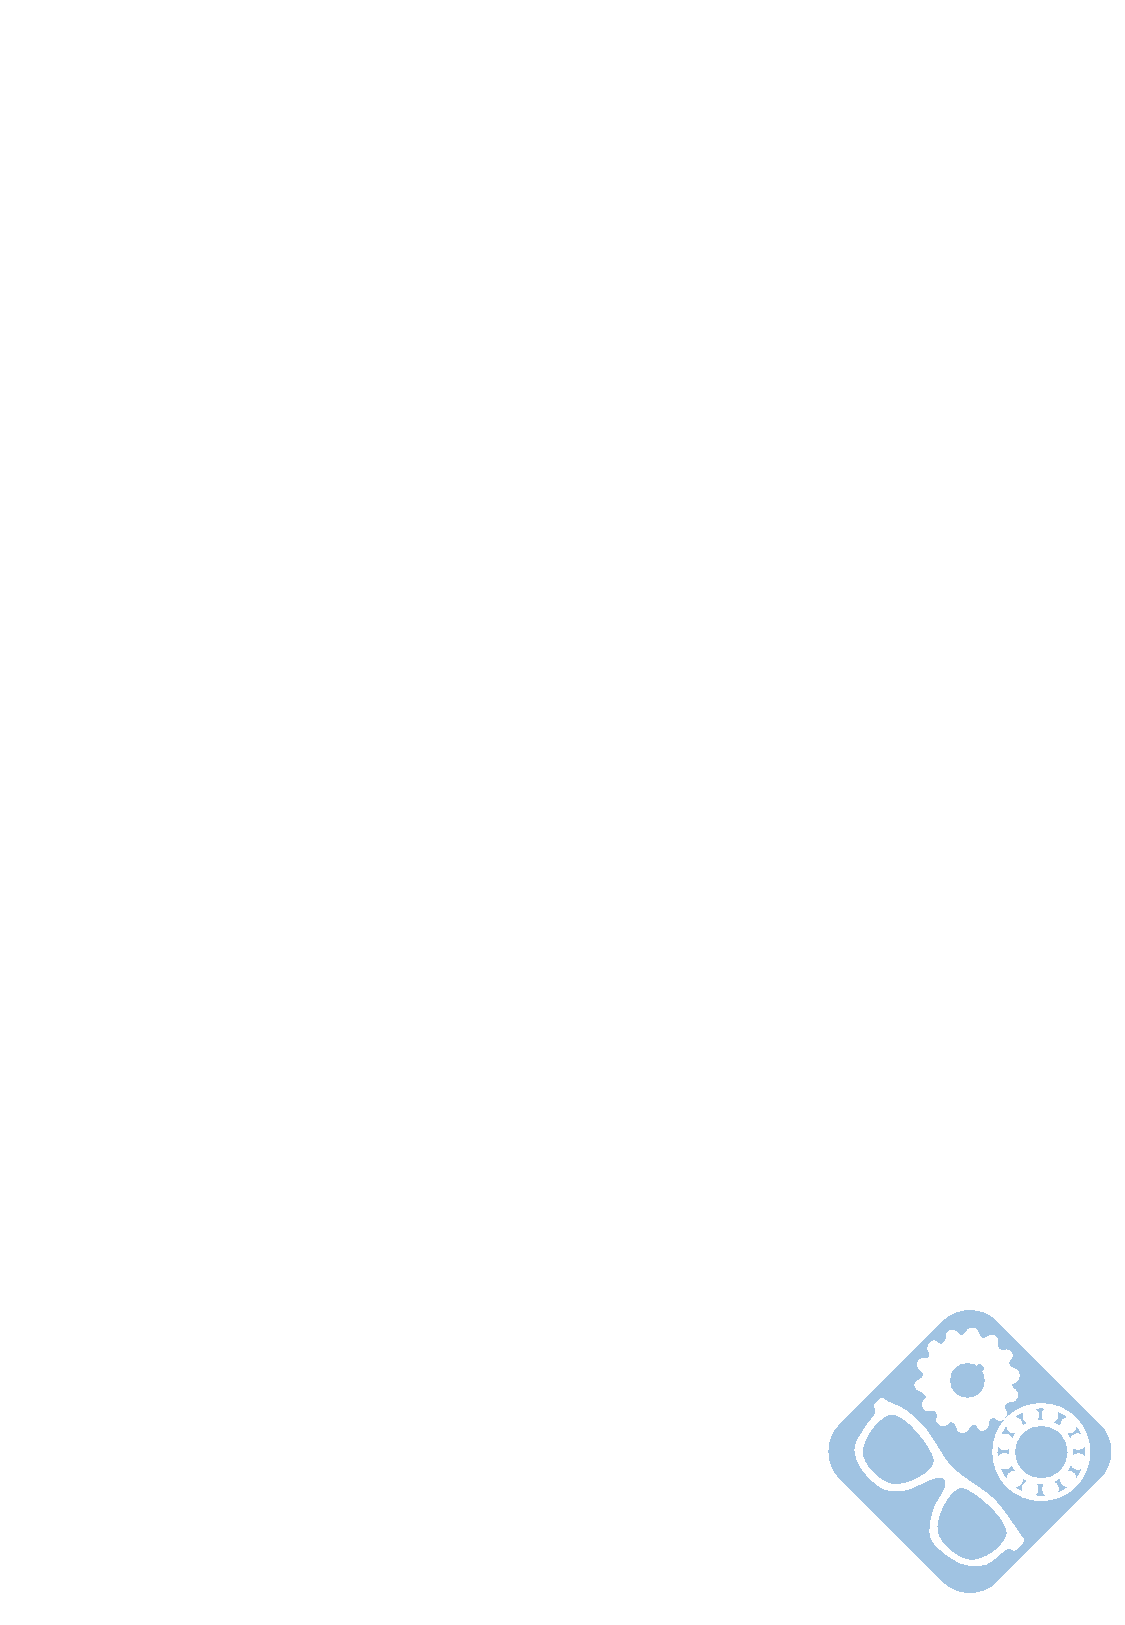
\includegraphics[width=\paperwidth,height=\paperheight,%
keepaspectratio]{../../img/fond4}%
\end{center}
\vfill
}}}

\begin{document}

\pagestyle{empty}

\vspace*{-3\baselineskip}

\AddToShipoutPicture*{\BackgroundPic}

\ifdef{\auteurdeux}{\begin{tabular}{>{\columncolor{gray!00}}m{.3\linewidth} m{.3\linewidth} >{\columncolor{gray!00}}m{.3\linewidth}}
Séquence : \sequence &  \multirow{3}{*}{\hspace{1cm}
\includegraphics[height=1.5cm]{../../img/logo}} &  \begin{flushright} \multirow{4}{*}{\hspace{1cm}
\includegraphics[height=4cm]{img/qrcode}}\end{flushright}\\
Document : \type\num \\
 \institute \\
 \auteurun\\
 \auteurdeux
\end{tabular}}{\begin{tabular}{>{\columncolor{gray!00}}m{.3\linewidth} m{.3\linewidth} >{\columncolor{gray!00}}m{.3\linewidth}}
Séquence : \sequence &  \multirow{3}{*}{\hspace{1cm}
\includegraphics[height=1.5cm]{../../img/logo}} &  \begin{flushright} \multirow{4}{*}{\hspace{1cm}
\includegraphics[height=4cm]{img/qrcode}}\end{flushright}\\
Document : \type\num \\
 \institute \\
 \auteurun
\end{tabular}}

\vspace{1cm}

\ifdef{\prive}{\begin{center}\colorbox{danger}{\Huge{Avec Correction}}\end{center}}{}

\begin{center}\huge{\nom}\end{center}

\vspace{2cm}

\ifdef{\imagedeux}{\begin{minipage}{0.49\linewidth}}{}
\begin{center}\includegraphics[height=5cm]{/home/renaud/Documents/Renaud/GitHub/django_education/systemes/\imageun}\end{center}
\ifdef{\imagedeux}{\end{minipage}\hfill
\begin{minipage}{0.49\linewidth}
\begin{center}\includegraphics[height=5cm]{/home/renaud/Documents/Renaud/GitHub/django_education/systemes/\imagedeux}\end{center}
\end{minipage}}{}

\vspace{5cm}


\begin{tabular}{p{.15\linewidth} >{\columncolor{white}}p{.8\linewidth}}
    \rowcolor{gray!20}
    Référence & S\sequence\ - \type\num \\
    Compétences & \competences \\
 	\rowcolor{gray!20}
    Description & \descrip \\
    Système & \systemes
  \end{tabular}

\newpage

\AddToShipoutPicture{\BackgroundPicdeux}

\pagestyle{normal}

\section{Assemblage vissé}

\subsection{Présentation}

L'exercice va consister en la mise en place de chaînes de cotes 2D afin de garantir une liste d'exigences géométriques.

\begin{center}
 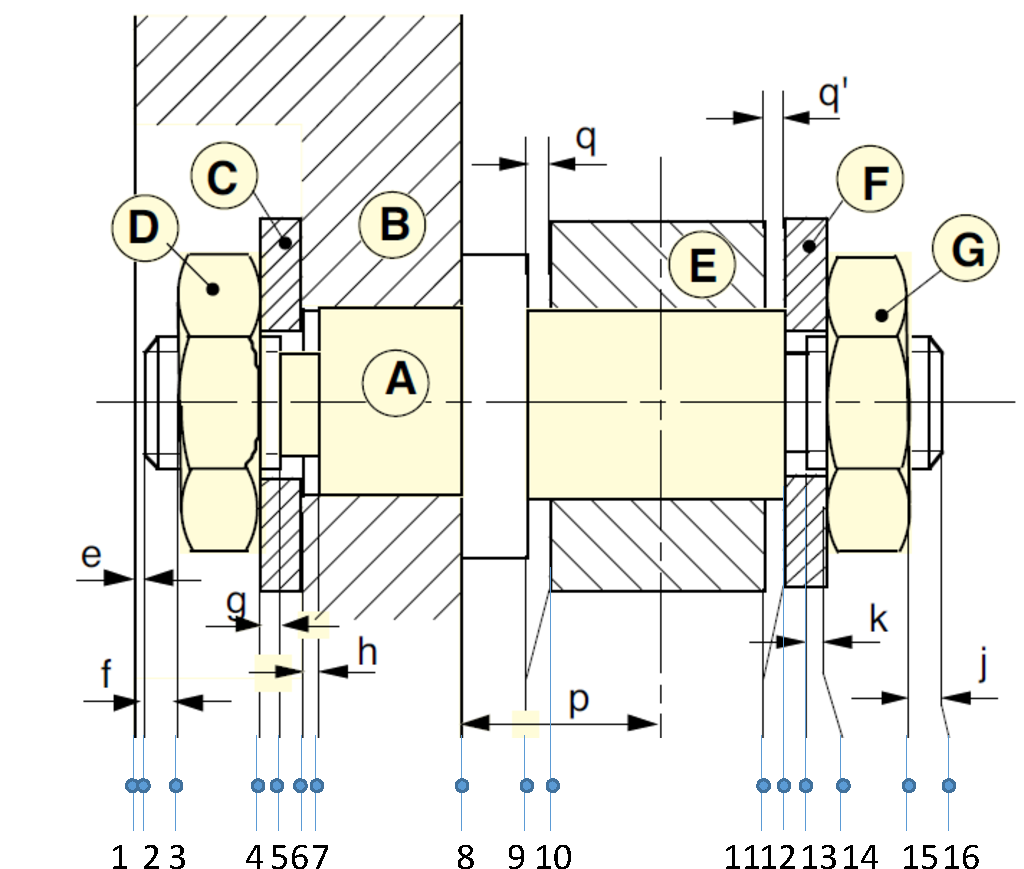
\includegraphics[width=0.7\linewidth]{img/Specifs_num}
\end{center}

Exigences:
\begin{itemize}
 \item un jeu mini de $0,2mm$ entre le galet E et ses pièces voisines A et F
 
 $q'_{mini} = 0,2$ et  $q_{mini} = 0,2$
 \item un déplacement maxi de $1,2mm$ du plan de symétrie du galet E par rapport a B

 $IT p = 1,2$ 
 \item un dépassement de $4mm$ mini des 2 têtes de filetage de l'arbre A des écrous G et D

 $j_{mini} = 4$ et $f mini = 4$
 \item h une longueur des deux filetages de l'arbre A suffisante pour que les écrous G et D soient toujours en prise sur leur filetage
 
 $g mini = 1$
 $k mini = 1$
 \item h un serrage entre les pièces A et B

 $h mini = 1$
 \item h un retrait de $0,5mm$ mini de la tête de l'arbre A par rapport a la pièce B

 $e mini = 0,5$
\end{itemize}

\newpage

\subsection{Écriture des spécifications}

\begin{center}
 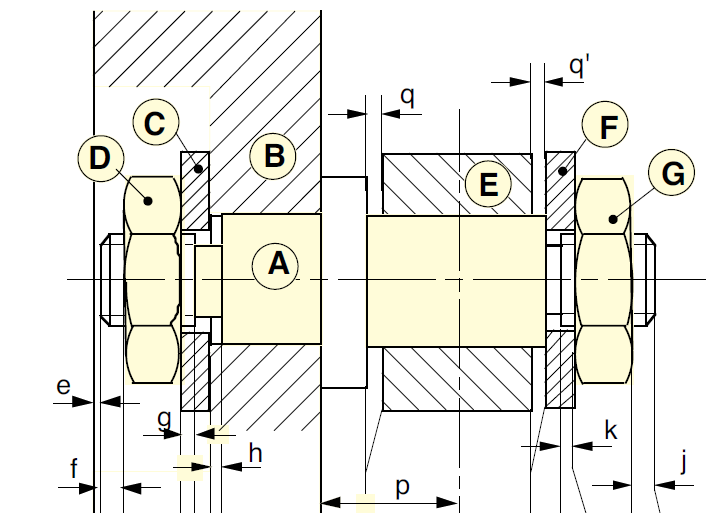
\includegraphics[width=0.7\linewidth]{img/Specif2}

\vspace{3cm}

 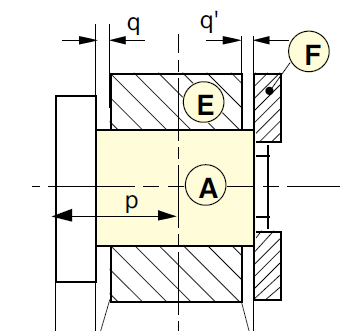
\includegraphics[width=0.4\linewidth]{img/Specif3.png}
\end{center}

\newpage

\begin{center}
 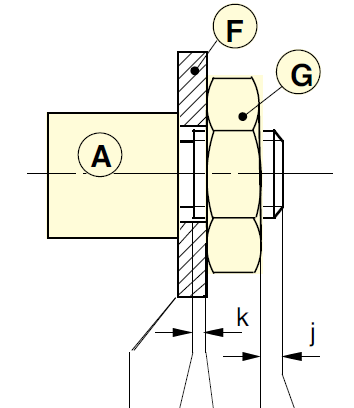
\includegraphics[width=0.4\linewidth]{img/Specif4.png}

\vspace{3cm}

 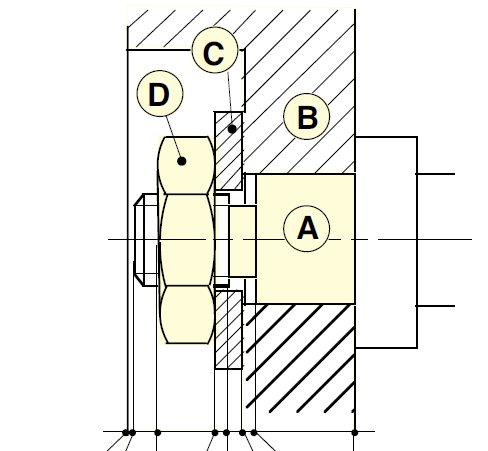
\includegraphics[width=0.5\linewidth]{img/Specif5.png}
\end{center}

\newpage

\begin{center}
 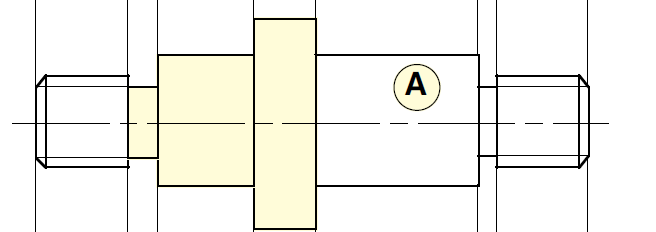
\includegraphics[width=0.7\linewidth]{img/Specif6.png}
\end{center}

\vspace{1cm}

\paragraph{Question 1:} Déterminer les chaînes de cotes qui permettent de respecter les exigences établies au-dessus.

\newpage

\section{Moteur}

\subsection{Présentation}

L'étude de ce sujet va porter sur l'assemblage d'un moteur. La méthode suivante permet de définir comment mettre les spécifications à partir de l'assemblage des différentes pièces.


\begin{minipage}{0.48\linewidth}
 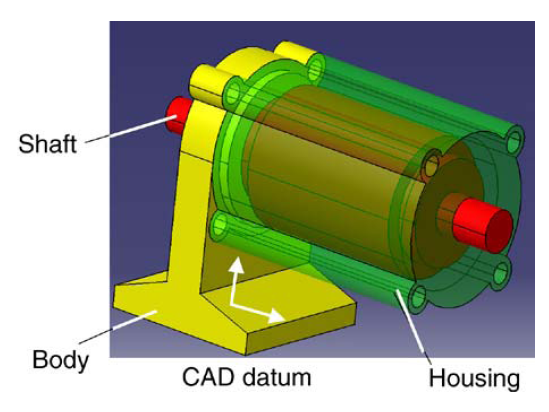
\includegraphics[width=0.9\linewidth]{img/Moteur1.png}
\end{minipage}
\hfill
\begin{minipage}{0.48\linewidth}
 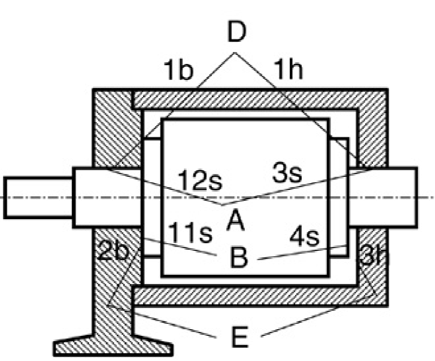
\includegraphics[width=0.9\linewidth]{img/Moteur2.png}
\end{minipage}

\subsection{Écriture des spécifications sur les pièces}

\begin{center}
 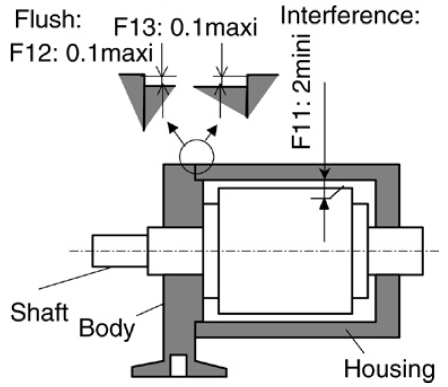
\includegraphics[width=0.5\linewidth]{img/Moteur3.png}
\end{center}

\newpage

\begin{center}
 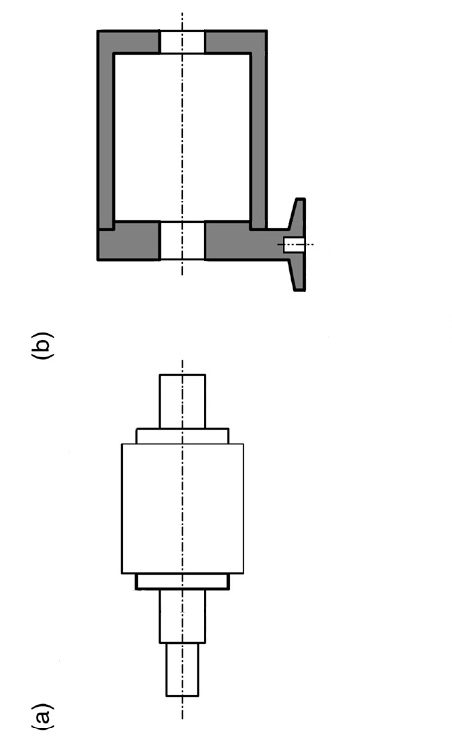
\includegraphics[width=0.5\linewidth,angle=270]{img/Moteur4.png}
\end{center}

\paragraph{Question 1:} Définir la mise en position du rotor.

\paragraph{Question 2:} Définir la spécification pour l'assemblage.

\paragraph{Question 3:} Définir la spécification liée aux exigences suivantes

\newpage

\section{Planeur sous-marin}

\subsection{Présentation}

\begin{minipage}{0.55\linewidth}
Traditionnellement, le milieu océanique est observé à l'aide d'instruments qui sont embarqués sur des navires océanographiques ou sur des flotteurs dérivant.

Le "planeur sous-marin" est une plate-forme très complémentaire des systèmes d'observation existants, particulièrement pour la surveillance de certaines régions clefs de l'océan. 
\end{minipage}
\hfill
\begin{minipage}{0.4\linewidth}
 \centering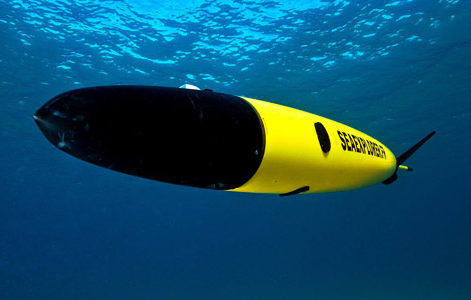
\includegraphics[width=0.8\linewidth]{img/Planeur.jpg}
\end{minipage}

\subsection{Performance hydrodynamique}

Les performances de mobilité du planeur (rayon d'action, vitesse, autonomie) sont liées à sa finesse qui doit être maximale. La finesse est la capacité à parcourir une grande distance avec un minimum de variation d'altitude.

Entre autres points, l'avant du planeur est un élément participant de façon importante à cette finesse. Le nez du planeur a ainsi été calculé par les hydrodynamiciens qui ont proposé une forme en « ogive » dont la courbe guide est décrite sur le tracé suivant.
\begin{center}
 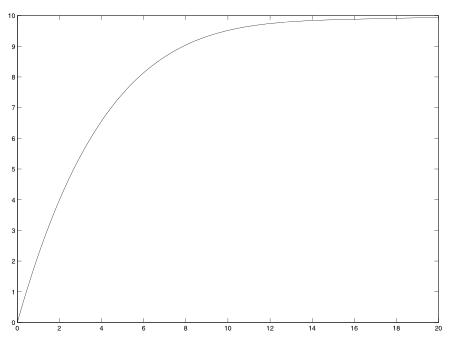
\includegraphics[width=0.6\linewidth]{img/Hydro.png}
\end{center}

La partie avant est réalisée par usinage sur Machine outil à commande numérique dans un alliage résistant au milieu marin traité par anodisation. L'anodisation dure 1 heure dans un sel de bichromate de potassium porté à 98°C. 

L'alliage utilisé est un $AlMg1SiCu$. Ses caractéristiques mécaniques sont les suivantes : $Rm=310MPa$, 
$E=68,9GPa$, $A\%=17$.

\paragraph{Question 1:} Quelle est la composition de l'alliage proposé ?

\paragraph{Question 2:} Tracer, en positionnant les valeurs caractéristiques, l'allure de la courbe de traction pour cet alliage.

\paragraph{Question 3:} Expliquer les spécifications portées sur le dessin de définition de la figure \ref{plan}.

\paragraph{Question 4:} Proposer une cotation normalisée entre les deux plans B et C qui permette de positionner les deux surfaces (voir figure \ref{plan}, valeur nominale 10 mm, IT = 0,2 mm).

\begin{figure}[!h]
 \centering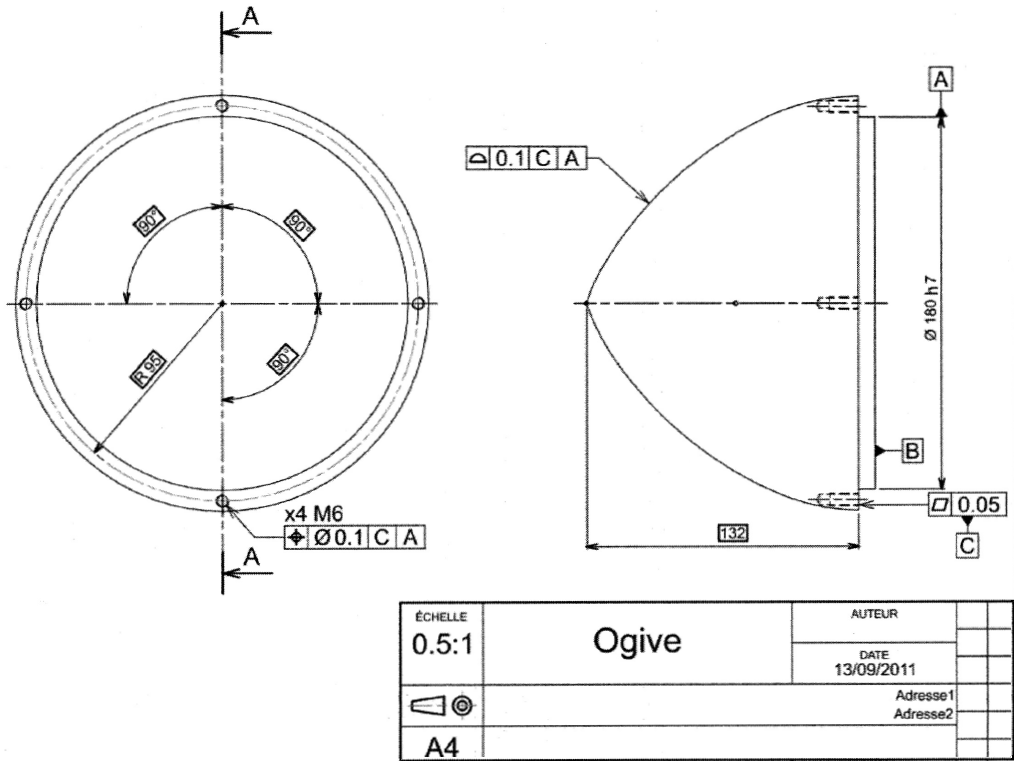
\includegraphics[width=\linewidth]{img/Plan_sous_marin.png}
 \caption{Plan de l'ogive}
 \label{plan}
\end{figure}

\newpage

\section{Roue motrice de chariot élévateur}

\begin{minipage}{0.65\linewidth}
Le chariot élévateur, objet de cette étude, est utilisé pour la manutention et le stockage des
marchandises dans des entrepôts. Il comporte trois roues : deux situées à l'avant sont dites porteuses et la troisième, située à l'arrière, est à la fois motrice et directrice.
\end{minipage}\hfill
\begin{minipage}{0.3\linewidth}
\centering 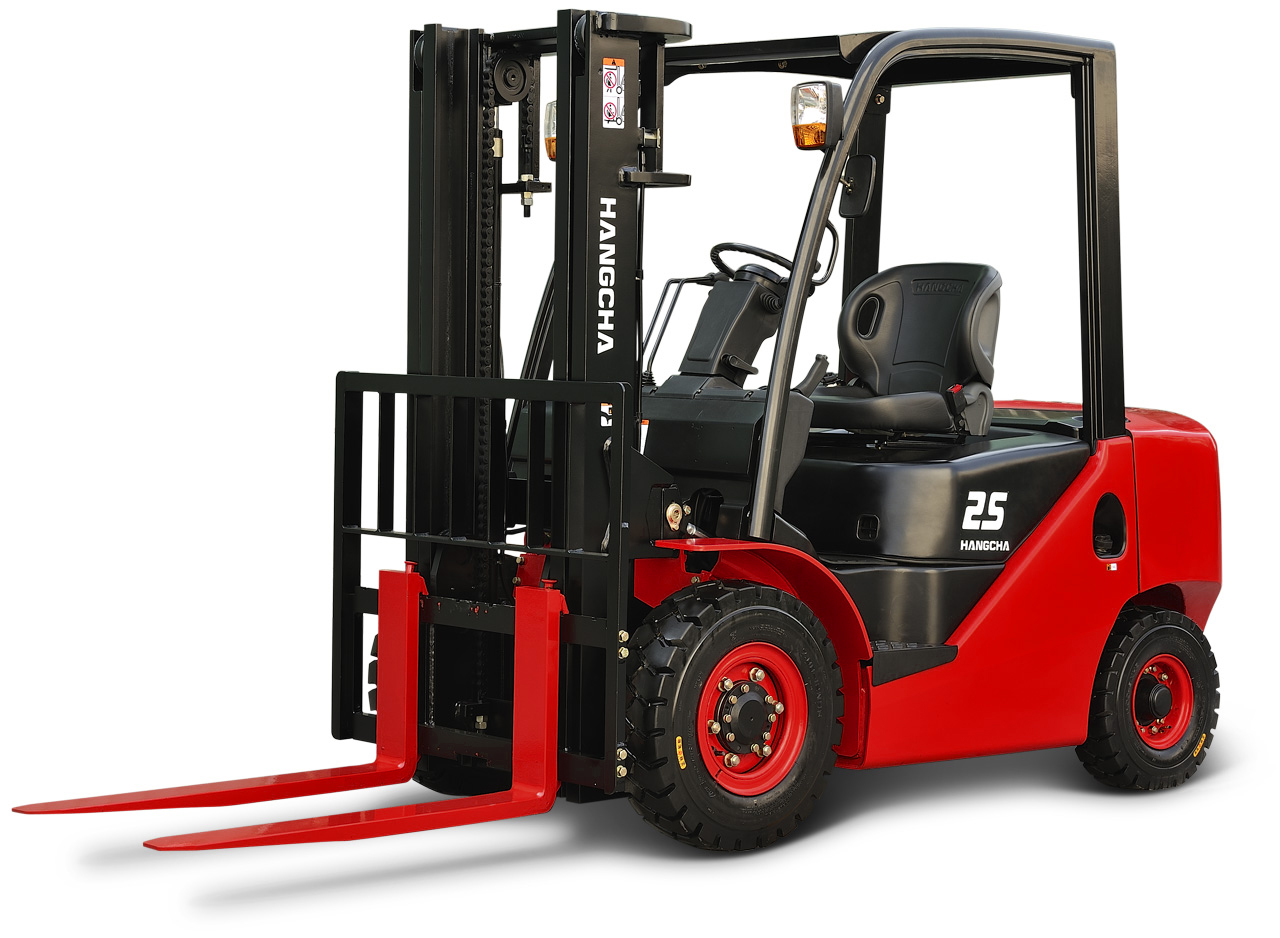
\includegraphics[width=0.8\linewidth]{img/XF25}
\end{minipage}

Une vue en coupe et en perspective de la roue permet de découvrir sa conception intérieure.

\begin{center}
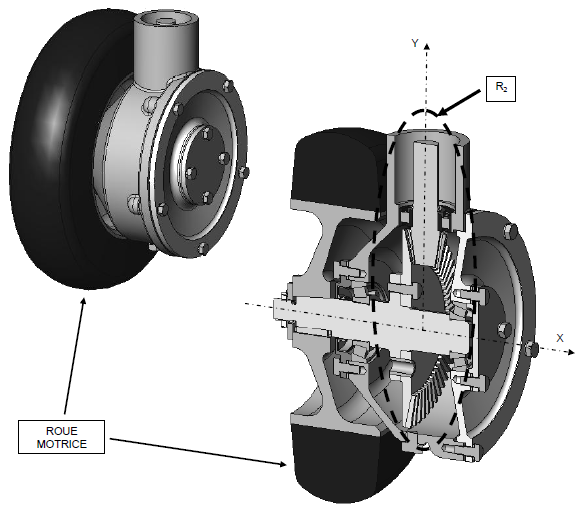
\includegraphics[width=0.8\linewidth]{img/roue1}
\end{center}

La vue éclatée permet de distinguer les pièces assemblées pour ce mécanisme.

\begin{center}
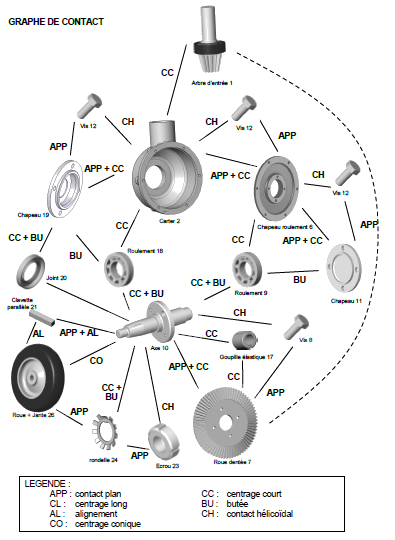
\includegraphics[width=\linewidth]{img/roue2}
\end{center}

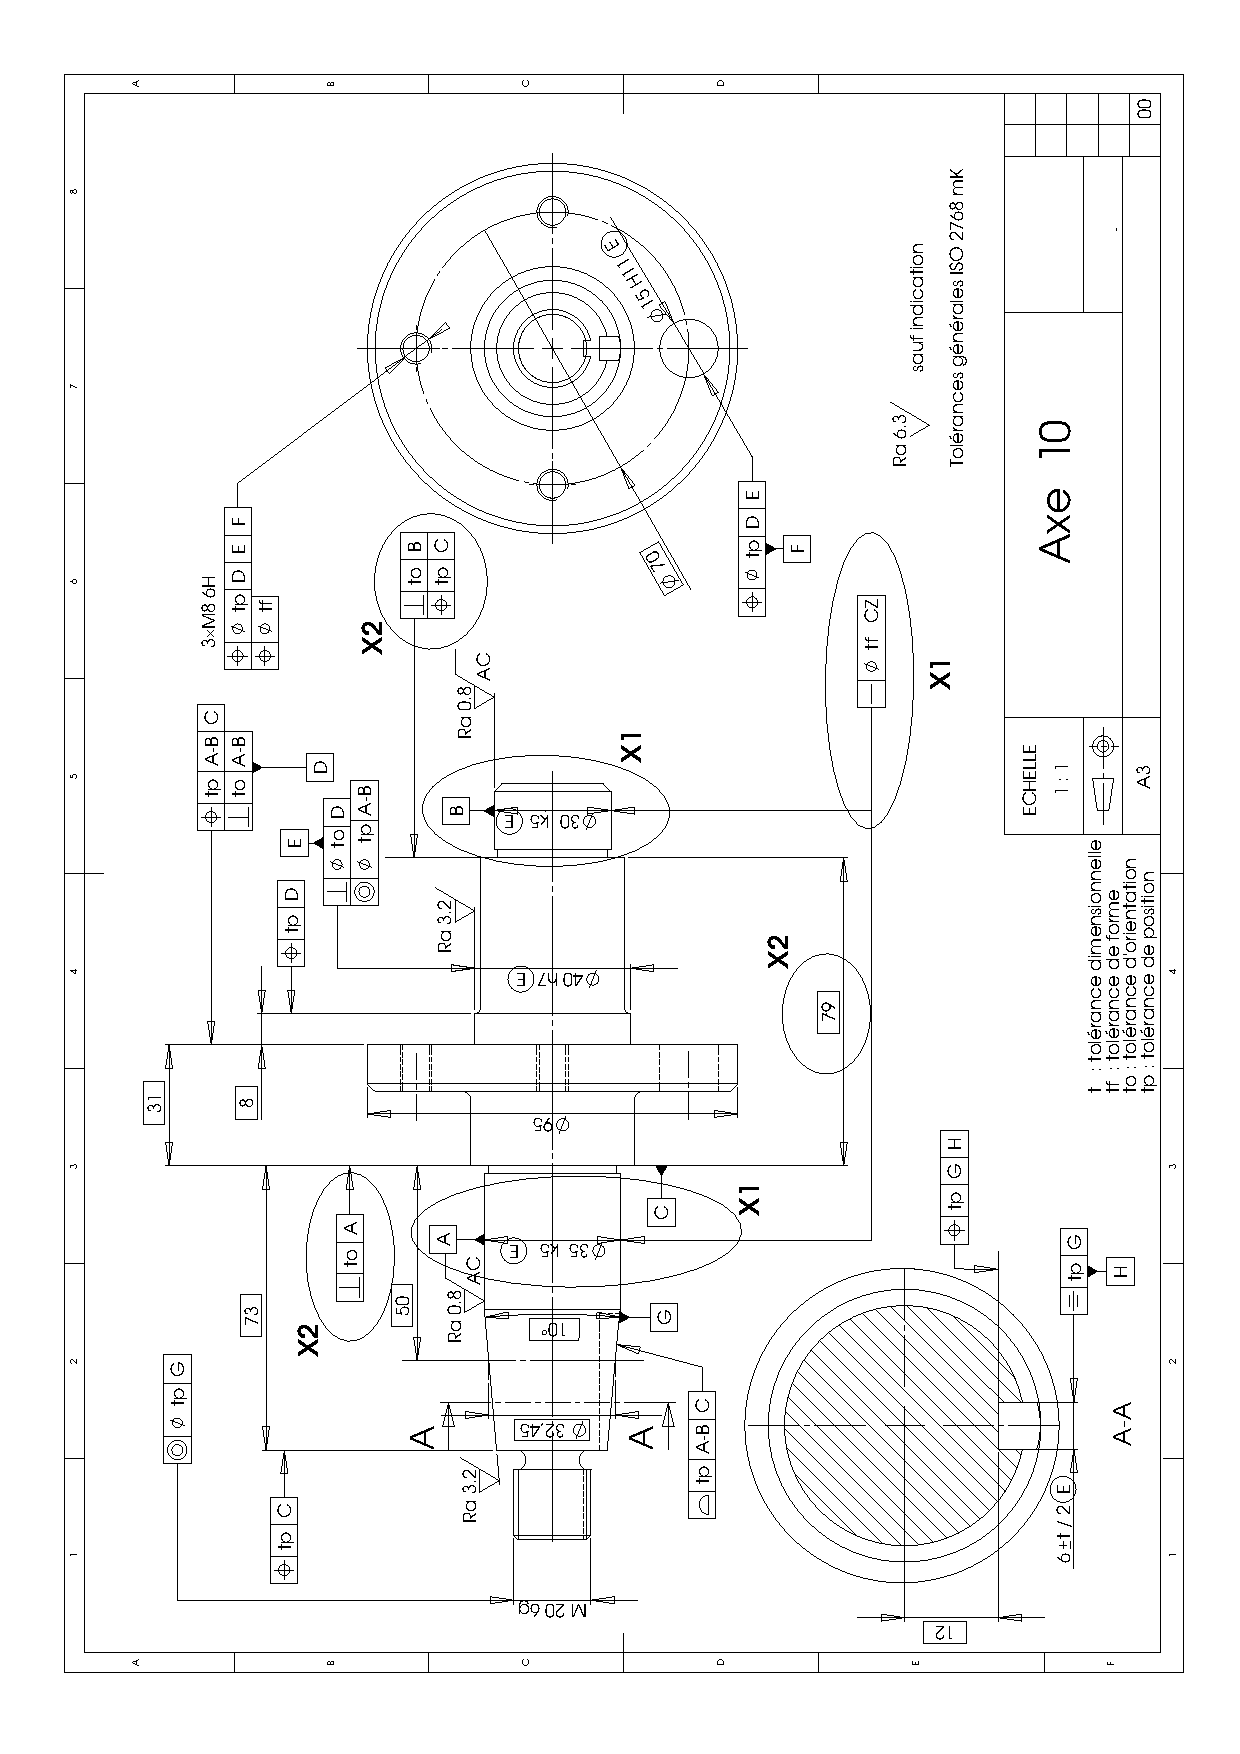
\includepdf{img/axe10cotationGPS}

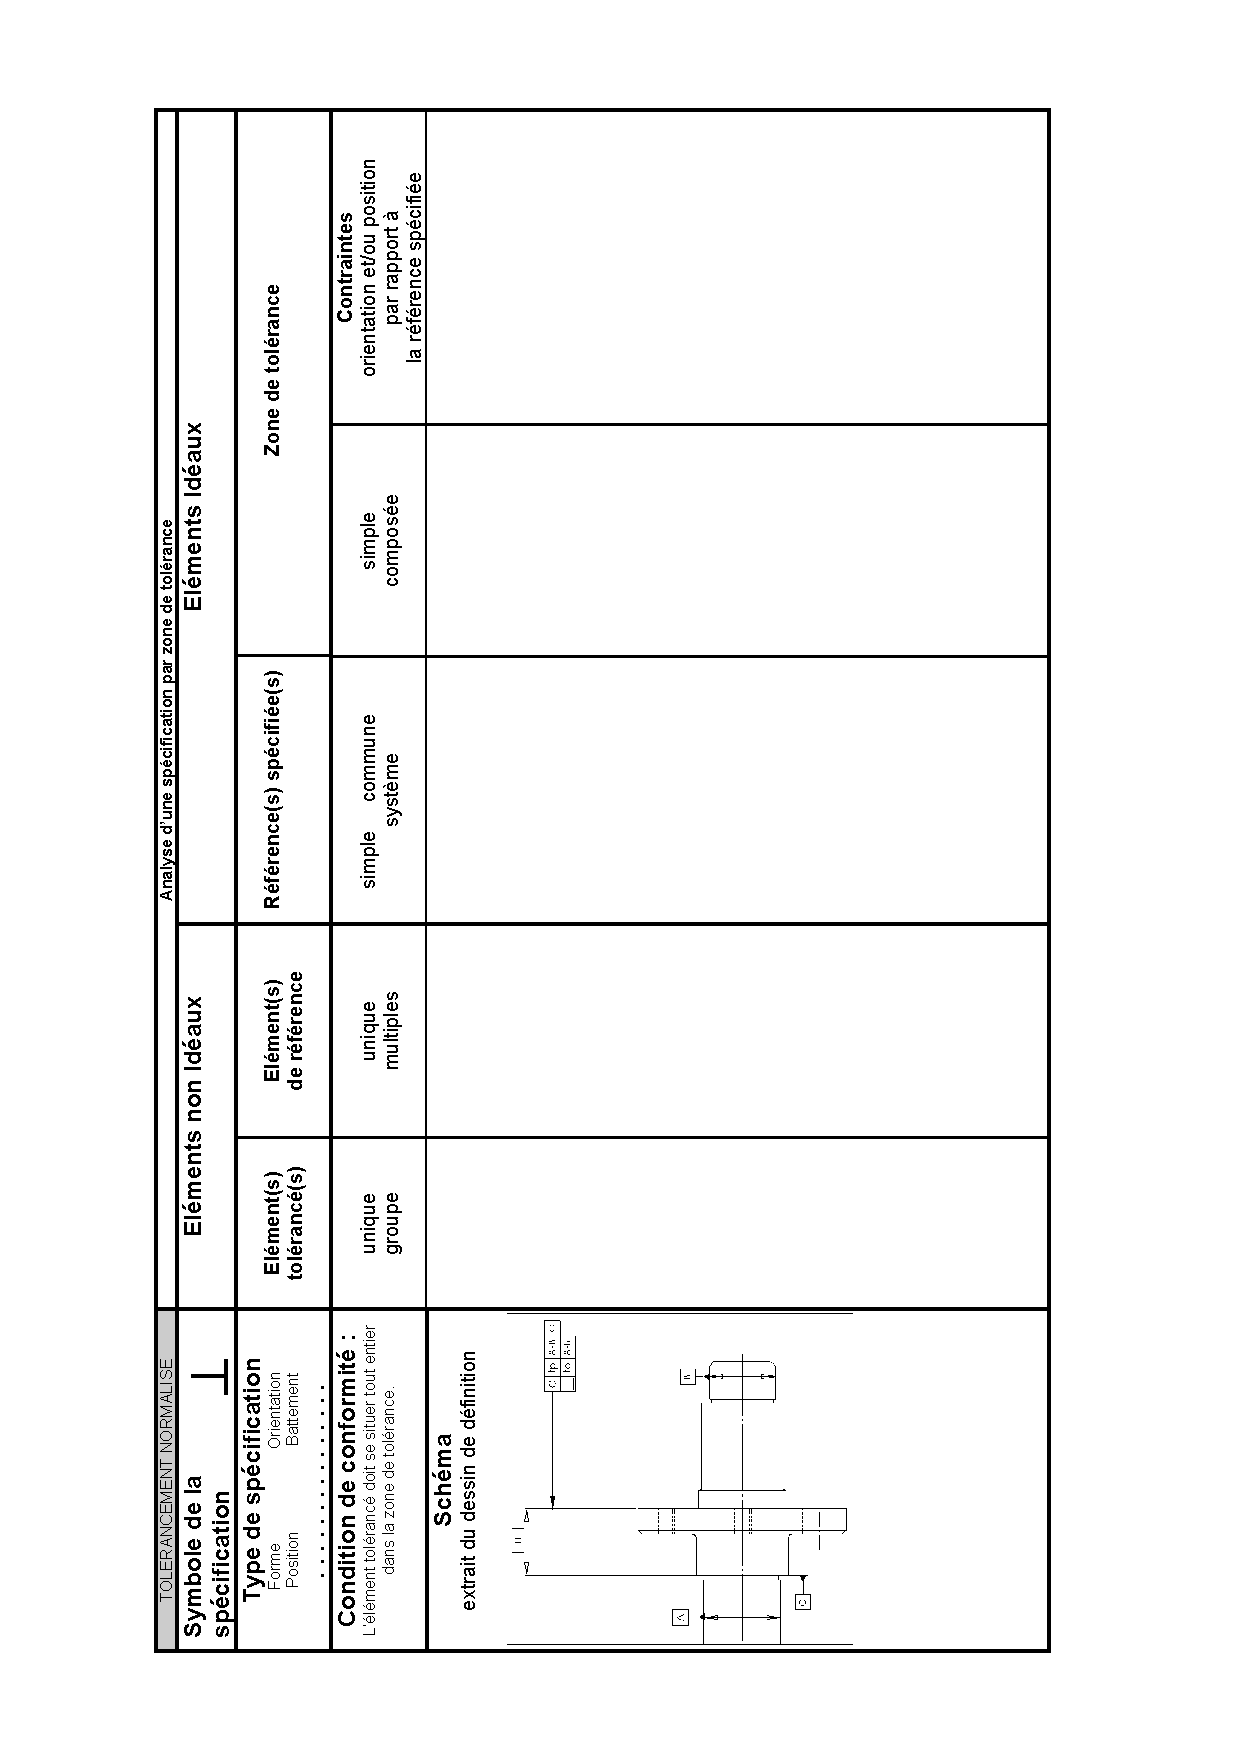
\includepdf{img/axe10cotationGPS2}

\end{document}
\clearpage

\ifdef{\public}{\end{document}}{}

\newpage

\pagestyle{correction}

\section{Correction}

\subsection{Assemblage vissé}

\begin{itemize}
 \item q,q': $A_{9,12}min-E_{10,11}max\geq 0.4$,
 \item p: $A_{9,12}max-E_{10,11}min\leq 1.2$,
 \item j: $A_{12,16}min-F_{12,14}max-G_{14,15}max\geq 4$,
 \item f: $A_{2,8}min-B_{6,8}max-C_{4,6}max-D_{3,4}max\geq 4$,
 \item g: $C_{4,6}min+B_{6,8}min-A_{5,8}max\gep 1$,
 \item k: $F_{12,14}min-A_{12,13}max\gep 1$,
 \item h: $B_{6,8}min-A_{7,8}max\gep 1$,
 \item e: $B_{1,8}min-A_{2,8}max\gep 0.5$.
\end{itemize}



\end{document}
